\documentclass[a4paper]{report}

% load packages
%\usepackage{showframe}
\usepackage[utf8]{inputenc}
\usepackage{enumitem}
\usepackage{listings}
\usepackage{courier}
\usepackage{hyperref}
\usepackage{graphicx}
\usepackage{float}
\usepackage[export]{adjustbox}

\setlength{\parskip}{1em}

\lstset{
  breaklines=true,
  basicstyle=\ttfamily,
  showstringspaces=false
}

\begin{document}

\title{Report of Programming Assignment 2 for CS 6301.001: Special Topics in Computer Science --- Introduction to Multi-Core Programming}

\author{Siming Liu}

\maketitle{}

\section*{Experiment Objective}
The experiment is intended to compare performance of three different implementations of concurrent linked lists. There are coarse-grained locking, fine-grained locking using lazy-synchronization and lock-free.

\section*{Experimental Environment}
Experiments run on a visualization node of \href{https://www.tacc.utexas.edu/}{TACC} distributed supercomputer clusters.
A visualization node have 2 Intel Xeon E5-2680 processors (x86\_64 architecture, 16 total cores) and 32GB of memory.
The operating system of a node runs is CentOS 6.8 with Linux kernel version 2.6.32.
Programming language of implementation is \lstinline{C++}.
The performance is compared with respect to system throughput with two parameters:
\begin{enumerate}
  \item distribution of various operations:
  \begin{itemize}
    \item read-dominated: 90\% search, 9\% insert and 1\% delete
    \item mixed: 70\% search, 20\% insert and 10\% delete
    \item write-dominated: 0\% search, 50\% insert and 50\% delete
  \end{itemize}
  \item degree of concurrency: it varies the number of threads from one to twice the number of cores in a node. (aka $1 \sim 32$)
\end{enumerate}

\section*{Experimental Method}
In order to limit the maximum size of list to 1000 keys, we set the maximum operations number to 2000.
For each type of throughput, we randomly generate 2000 operations according to the profile and then distribute these operations randomly to each thread as parameter. For each implementation, we launch $1 \sim 32$ threads to execution all 2000 operations and we do this 16 times to get average running time of all threads in nanosecond. And in order to add degree of contention, we limit the key space small which is from 0 to 9. So command \lstinline{concurrent_linked_list 32 2000 16 9} are used to launch testing, in which 32 is maximum thread number, 2000 is operation number, 16 is repeated times and 9 is maximum key value.

\section*{How to Test Correctness}
For each operation of each thread, we log on the invocation and response event. The macro \lstinline{CALL_FUNC_IF_MATCH} is intended for this logging. So for each unit test, we can get a concurrent history of all threads. And we manually check all concurrent histories to see whether they are all linearizability. If all the concurrent histories tested of a implementation are linearizability, we can say the implementation is correct with high probability. In order to achieve that and conveniently for manually checking, we use command \lstinline{concurrent_linked_list 5 20 1 4} to test correctness. Noted that in the parameter, we keep key space very small to highly increase degree of contention.

\section*{Experiment Results}
For each throughput, we generate a plot to compare three implementation's performance. Here they are.
\begin{figure}[H]
  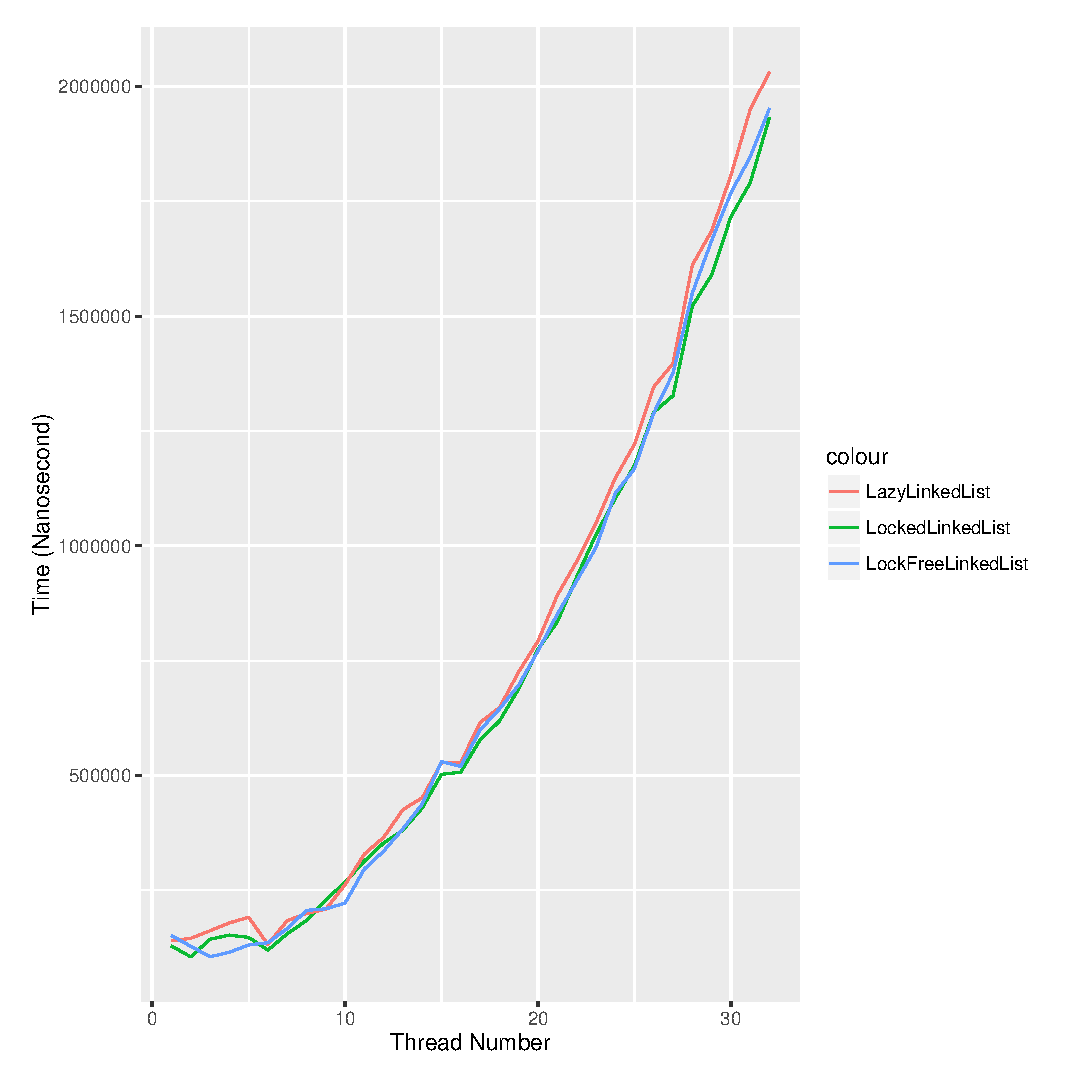
\includegraphics[scale=0.8]{result/result-tacc-7796986-read}
  \caption{Read-dominated Throughput}
\end{figure}

\begin{figure}[H]
  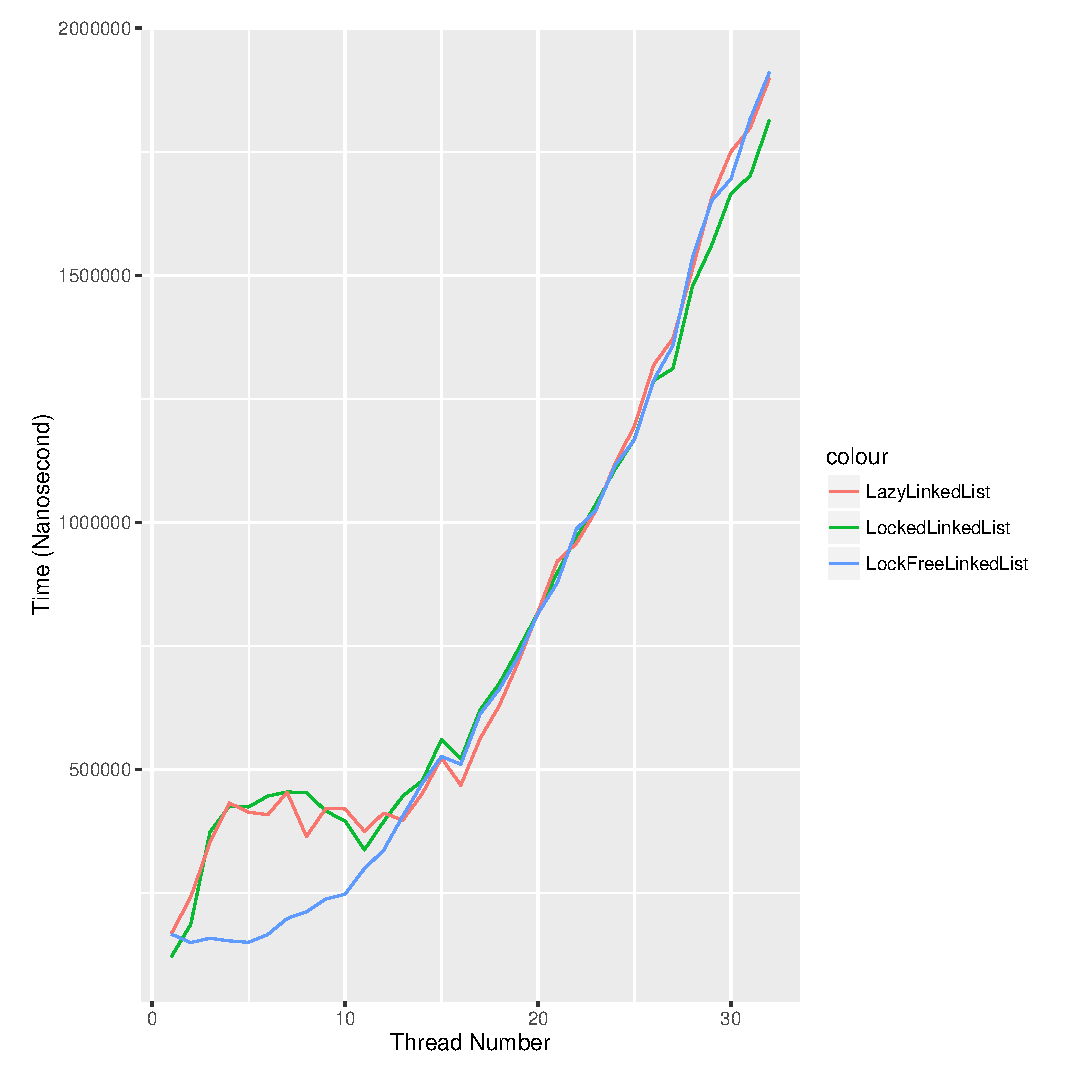
\includegraphics[scale=0.8]{result/result-tacc-7796986-mixed}
  \caption{Mixed Throughput}
\end{figure}

\begin{figure}[H]
  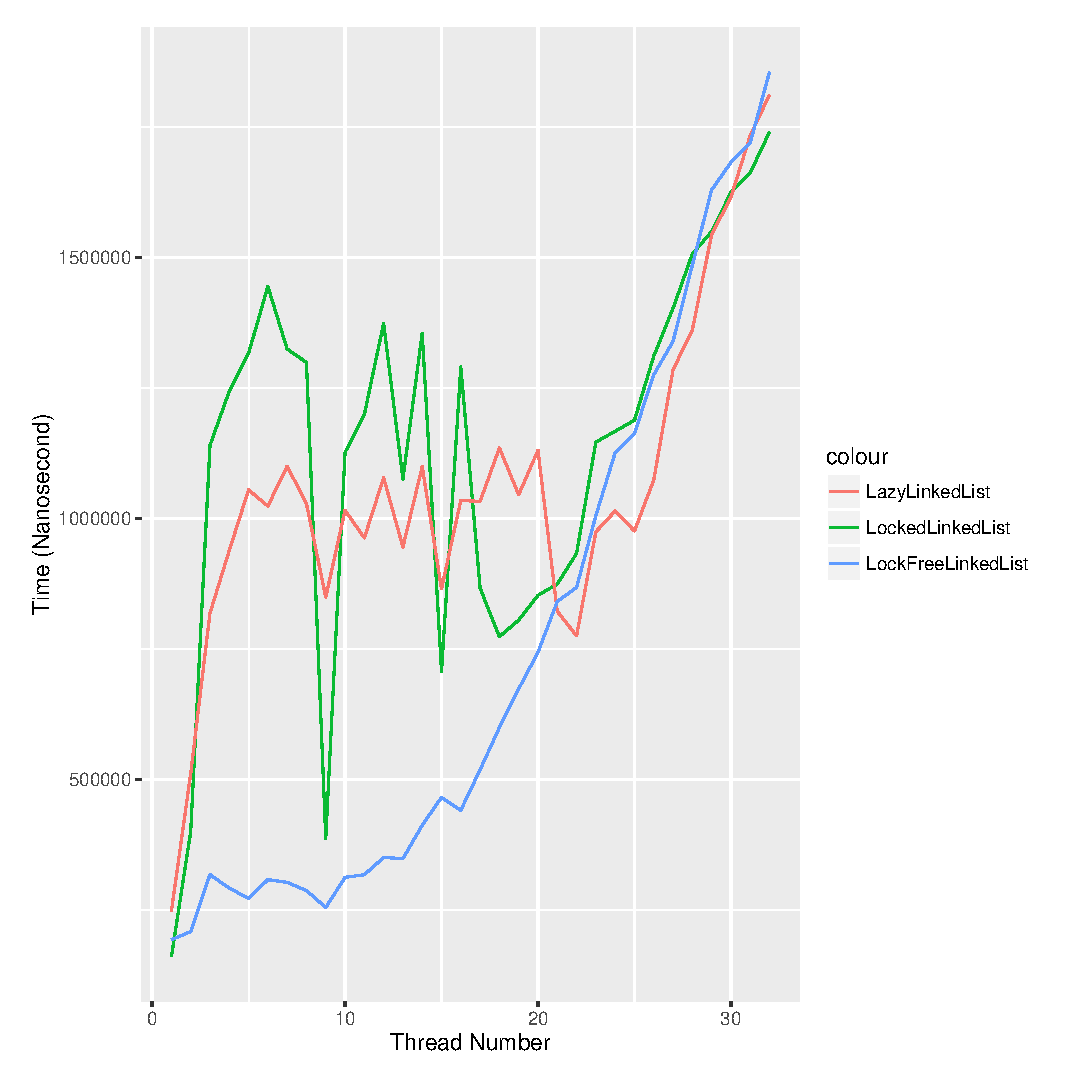
\includegraphics[scale=0.8]{result/result-tacc-7796986-write}
  \caption{Write-dominated Throughput}
\end{figure}

\section*{Results Analysis}
We discuss each throughput one by one.

In the read-dominated throughput, because 90\% operations are search and search function in all three implementations are lock-free, so basically all implementations in this throughput performs the same. The plot is as expected.

In the mixed throughput, when threads number varies from 1 to 16, in this situation, each thread could run on a core of CPU. So the lock-free linked lists performs best. When the threads number goes beyond 16, some core must switch different threads in the running. This switching is time-consuming. In this situation and because 70\% operations remains search operation, all implementations performs the same. The plot is as expected.

In the write-dominated throughput, there is no search operations. So this throughput will distinct the performance of three implementations. We can see that the performance behavior are distinct clearly before threads number goes beyond 20. It is lock-free $>$ lazy synchronization $>$ coarse-grained as expected. And when threads number goes beyond 20, they all performs basically the same and even lock-free loses advantages because thread switching becomes dominate.

\end{document}
